% REV01 Wed 23 Jun 2021 06:42:54 WIB
% START Tue 04 May 2021 13:55:16 WIB

\chapter{MORE BIRDS OF PREY}

Rogue Riderhood dwelt deep and dark in Limehouse Hole, among the
riggers, and the mast, oar and block makers, and the boat-builders, and
the sail-lofts, as in a kind of ship’s hold stored full of waterside
characters, some no better than himself, some very much better, and
none much worse. The Hole, albeit in a general way not over nice in
its choice of company, was rather shy in reference to the honour of
cultivating the Rogue’s acquaintance; more frequently giving him the
cold shoulder than the warm hand, and seldom or never drinking with him
unless at his own expense. A part of the Hole, indeed, contained so
much public spirit and private virtue that not even this strong leverage
could move it to good fellowship with a tainted accuser. But, there may
have been the drawback on this magnanimous morality, that its exponents
held a true witness before Justice to be the next unneighbourly and
accursed character to a false one.

Had it not been for the daughter whom he often mentioned, Mr Riderhood
might have found the Hole a mere grave as to any means it would yield
him of getting a living. But Miss Pleasant Riderhood had some little
position and connection in Limehouse Hole. Upon the smallest of small
scales, she was an unlicensed pawnbroker, keeping what was popularly
called a Leaving Shop, by lending insignificant sums on insignificant
articles of property deposited with her as security. In her
four-and-twentieth year of life, Pleasant was already in her fifth year
of this way of trade. Her deceased mother had established the business,
and on that parent’s demise she had appropriated a secret capital of
fifteen shillings to establishing herself in it; the existence of
such capital in a pillow being the last intelligible confidential
communication made to her by the departed, before succumbing to
dropsical conditions of snuff and gin, incompatible equally with
coherence and existence.

Why christened Pleasant, the late Mrs Riderhood might possibly have
been at some time able to explain, and possibly not. Her daughter had no
information on that point. Pleasant she found herself, and she couldn’t
help it. She had not been consulted on the question, any more than on
the question of her coming into these terrestrial parts, to want a name.
Similarly, she found herself possessed of what is colloquially termed
a swivel eye (derived from her father), which she might perhaps have
declined if her sentiments on the subject had been taken. She was not
otherwise positively ill-looking, though anxious, meagre, of a muddy
complexion, and looking as old again as she really was.

As some dogs have it in the blood, or are trained, to worry certain
creatures to a certain point, so--not to make the comparison
disrespectfully--Pleasant Riderhood had it in the blood, or had been
trained, to regard seamen, within certain limits, as her prey. Show
her a man in a blue jacket, and, figuratively speaking, she pinned him
instantly. Yet, all things considered, she was not of an evil mind or an
unkindly disposition. For, observe how many things were to be considered
according to her own unfortunate experience. Show Pleasant Riderhood a
Wedding in the street, and she only saw two people taking out a regular
licence to quarrel and fight. Show her a Christening, and she saw a
little heathen personage having a quite superfluous name bestowed upon
it, inasmuch as it would be commonly addressed by some abusive epithet:
which little personage was not in the least wanted by anybody, and would
be shoved and banged out of everybody’s way, until it should grow
big enough to shove and bang. 

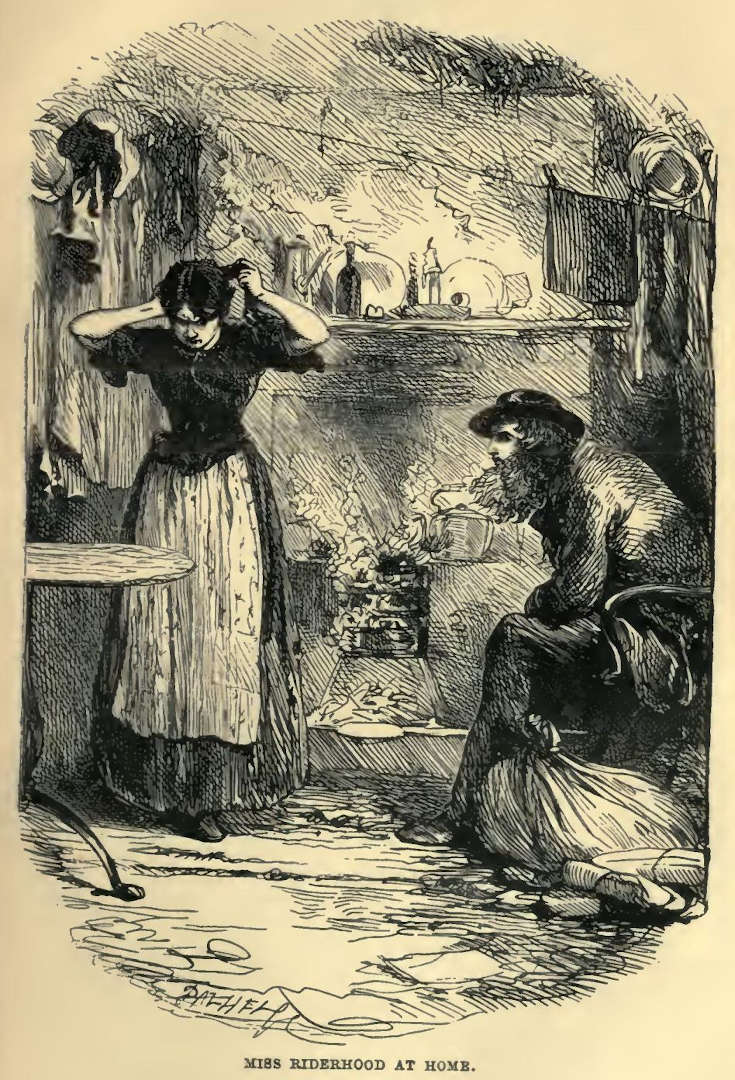
\includegraphics[scale=2.3]{02-12-01}

Show her a Funeral, and she saw an
unremunerative ceremony in the nature of a black masquerade, conferring
a temporary gentility on the performers, at an immense expense, and
representing the only formal party ever given by the deceased. Show her
a live father, and she saw but a duplicate of her own father, who from
her infancy had been taken with fits and starts of discharging his duty
to her, which duty was always incorporated in the form of a fist or a
leathern strap, and being discharged hurt her. All things considered,
therefore, Pleasant Riderhood was not so very, very bad. There was even
a touch of romance in her--of such romance as could creep into Limehouse
Hole--and maybe sometimes of a summer evening, when she stood with
folded arms at her shop-door, looking from the reeking street to the
sky where the sun was setting, she may have had some vaporous visions
of far-off islands in the southern seas or elsewhere (not being
geographically particular), where it would be good to roam with a
congenial partner among groves of bread-fruit, waiting for ships to be
wafted from the hollow ports of civilization. For, sailors to be got the
better of, were essential to Miss Pleasant’s Eden.

Not on a summer evening did she come to her little shop-door, when a
certain man standing over against the house on the opposite side of
the street took notice of her. That was on a cold shrewd windy evening,
after dark. Pleasant Riderhood shared with most of the lady inhabitants
of the Hole, the peculiarity that her hair was a ragged knot, constantly
coming down behind, and that she never could enter upon any undertaking
without first twisting it into place. At that particular moment, being
newly come to the threshold to take a look out of doors, she was winding
herself up with both hands after this fashion. And so prevalent was the
fashion, that on the occasion of a fight or other disturbance in the
Hole, the ladies would be seen flocking from all quarters universally
twisting their back-hair as they came along, and many of them, in the
hurry of the moment, carrying their back-combs in their mouths.

It was a wretched little shop, with a roof that any man standing in it
could touch with his hand; little better than a cellar or cave, down
three steps. Yet in its ill-lighted window, among a flaring handkerchief
or two, an old peacoat or so, a few valueless watches and compasses, a
jar of tobacco and two crossed pipes, a bottle of walnut ketchup, and
some horrible sweets these creature discomforts serving as a blind to
the main business of the Leaving Shop--was displayed the inscription
SEAMAN’S BOARDING-HOUSE.

Taking notice of Pleasant Riderhood at the door, the man crossed so
quickly that she was still winding herself up, when he stood close
before her.

‘Is your father at home?’ said he.

‘I think he is,’ returned Pleasant, dropping her arms; ‘come in.’

It was a tentative reply, the man having a seafaring appearance. Her
father was not at home, and Pleasant knew it. ‘Take a seat by the fire,’
were her hospitable words when she had got him in; ‘men of your calling
are always welcome here.’

‘Thankee,’ said the man.

His manner was the manner of a sailor, and his hands were the hands of
a sailor, except that they were smooth. Pleasant had an eye for sailors,
and she noticed the unused colour and texture of the hands, sunburnt
though they were, as sharply as she noticed their unmistakable looseness
and suppleness, as he sat himself down with his left arm carelessly
thrown across his left leg a little above the knee, and the right arm
as carelessly thrown over the elbow of the wooden chair, with the hand
curved, half open and half shut, as if it had just let go a rope.

‘Might you be looking for a Boarding-House?’ Pleasant inquired, taking
her observant stand on one side of the fire.

‘I don’t rightly know my plans yet,’ returned the man.

‘You ain’t looking for a Leaving Shop?’

‘No,’ said the man.

‘No,’ assented Pleasant, ‘you’ve got too much of an outfit on you for
that. But if you should want either, this is both.’

‘Ay, ay!’ said the man, glancing round the place. ‘I know. I’ve been
here before.’

‘Did you Leave anything when you were here before?’ asked Pleasant, with
a view to principal and interest.

‘No.’ The man shook his head.

‘I am pretty sure you never boarded here?’

‘No.’ The man again shook his head.

‘What DID you do here when you were here before?’ asked Pleasant. ‘For I
don’t remember you.’

‘It’s not at all likely you should. I only stood at the door, one
night--on the lower step there--while a shipmate of mine looked in to
speak to your father. I remember the place well.’ Looking very curiously
round it.

‘Might that have been long ago?’

‘Ay, a goodish bit ago. When I came off my last voyage.’

‘Then you have not been to sea lately?’

‘No. Been in the sick bay since then, and been employed ashore.’

‘Then, to be sure, that accounts for your hands.’

The man with a keen look, a quick smile, and a change of manner, caught
her up. ‘You’re a good observer. Yes. That accounts for my hands.’

Pleasant was somewhat disquieted by his look, and returned it
suspiciously. Not only was his change of manner, though very sudden,
quite collected, but his former manner, which he resumed, had a
certain suppressed confidence and sense of power in it that were half
threatening.

‘Will your father be long?’ he inquired.

‘I don’t know. I can’t say.’

‘As you supposed he was at home, it would seem that he has just gone
out? How’s that?’

‘I supposed he had come home,’ Pleasant explained.

‘Oh! You supposed he had come home? Then he has been some time out?
How’s that?’

‘I don’t want to deceive you. Father’s on the river in his boat.’

‘At the old work?’ asked the man.

‘I don’t know what you mean,’ said Pleasant, shrinking a step back.
‘What on earth d’ye want?’

‘I don’t want to hurt your father. I don’t want to say I might, if I
chose. I want to speak to him. Not much in that, is there? There shall
be no secrets from you; you shall be by. And plainly, Miss Riderhood,
there’s nothing to be got out of me, or made of me. I am not good for
the Leaving Shop, I am not good for the Boarding-House, I am not good
for anything in your way to the extent of sixpenn’orth of halfpence. Put
the idea aside, and we shall get on together.’

‘But you’re a seafaring man?’ argued Pleasant, as if that were a
sufficient reason for his being good for something in her way.

‘Yes and no. I have been, and I may be again. But I am not for you.
Won’t you take my word for it?’

The conversation had arrived at a crisis to justify Miss Pleasant’s hair
in tumbling down. It tumbled down accordingly, and she twisted it up,
looking from under her bent forehead at the man. In taking stock of his
familiarly worn rough-weather nautical clothes, piece by piece, she took
stock of a formidable knife in a sheath at his waist ready to his hand,
and of a whistle hanging round his neck, and of a short jagged knotted
club with a loaded head that peeped out of a pocket of his loose
outer jacket or frock. He sat quietly looking at her; but, with these
appendages partially revealing themselves, and with a quantity
of bristling oakum-coloured head and whisker, he had a formidable
appearance.

‘Won’t you take my word for it?’ he asked again.

Pleasant answered with a short dumb nod. He rejoined with another short
dumb nod. Then he got up and stood with his arms folded, in front of
the fire, looking down into it occasionally, as she stood with her arms
folded, leaning against the side of the chimney-piece.

‘To wile away the time till your father comes,’ he said,--‘pray is there
much robbing and murdering of seamen about the water-side now?’

‘No,’ said Pleasant.

‘Any?’

‘Complaints of that sort are sometimes made, about Ratcliffe and Wapping
and up that way. But who knows how many are true?’

‘To be sure. And it don’t seem necessary.’

‘That’s what I say,’ observed Pleasant. ‘Where’s the reason for it?
Bless the sailors, it ain’t as if they ever could keep what they have,
without it.’

‘You’re right. Their money may be soon got out of them, without
violence,’ said the man.

‘Of course it may,’ said Pleasant; ‘and then they ship again and get
more. And the best thing for ‘em, too, to ship again as soon as ever
they can be brought to it. They’re never so well off as when they’re
afloat.’

‘I’ll tell you why I ask,’ pursued the visitor, looking up from the
fire. ‘I was once beset that way myself, and left for dead.’

‘No?’ said Pleasant. ‘Where did it happen?’

‘It happened,’ returned the man, with a ruminative air, as he drew his
right hand across his chin, and dipped the other in the pocket of his
rough outer coat, ‘it happened somewhere about here as I reckon. I don’t
think it can have been a mile from here.’

‘Were you drunk?’ asked Pleasant.

‘I was muddled, but not with fair drinking. I had not been drinking, you
understand. A mouthful did it.’

Pleasant with a grave look shook her head; importing that she understood
the process, but decidedly disapproved.

‘Fair trade is one thing,’ said she, ‘but that’s another. No one has a
right to carry on with Jack in THAT way.’

‘The sentiment does you credit,’ returned the man, with a grim smile;
and added, in a mutter, ‘the more so, as I believe it’s not your
father’s.--Yes, I had a bad time of it, that time. I lost everything,
and had a sharp struggle for my life, weak as I was.’

‘Did you get the parties punished?’ asked Pleasant.

‘A tremendous punishment followed,’ said the man, more seriously; ‘but
it was not of my bringing about.’

‘Of whose, then?’ asked Pleasant.

The man pointed upward with his forefinger, and, slowly recovering that
hand, settled his chin in it again as he looked at the fire. Bringing
her inherited eye to bear upon him, Pleasant Riderhood felt more
and more uncomfortable, his manner was so mysterious, so stern, so
self-possessed.

‘Anyways,’ said the damsel, ‘I am glad punishment followed, and I say
so. Fair trade with seafaring men gets a bad name through deeds of
violence. I am as much against deeds of violence being done to seafaring
men, as seafaring men can be themselves. I am of the same opinion as my
mother was, when she was living. Fair trade, my mother used to say, but
no robbery and no blows.’ In the way of trade Miss Pleasant would have
taken--and indeed did take when she could--as much as thirty shillings
a week for board that would be dear at five, and likewise conducted the
Leaving business upon correspondingly equitable principles; yet she had
that tenderness of conscience and those feelings of humanity, that the
moment her ideas of trade were overstepped, she became the seaman’s
champion, even against her father whom she seldom otherwise resisted.

But, she was here interrupted by her father’s voice exclaiming angrily,
‘Now, Poll Parrot!’ and by her father’s hat being heavily flung from his
hand and striking her face. Accustomed to such occasional manifestations
of his sense of parental duty, Pleasant merely wiped her face on her
hair (which of course had tumbled down) before she twisted it up. This
was another common procedure on the part of the ladies of the Hole, when
heated by verbal or fistic altercation.

‘Blest if I believe such a Poll Parrot as you was ever learned to
speak!’ growled Mr Riderhood, stooping to pick up his hat, and making
a feint at her with his head and right elbow; for he took the delicate
subject of robbing seamen in extraordinary dudgeon, and was out of
humour too. ‘What are you Poll Parroting at now? Ain’t you got nothing
to do but fold your arms and stand a Poll Parroting all night?’

‘Let her alone,’ urged the man. ‘She was only speaking to me.’

‘Let her alone too!’ retorted Mr Riderhood, eyeing him all over. ‘Do you
know she’s my daughter?’

‘Yes.’

‘And don’t you know that I won’t have no Poll Parroting on the part of
my daughter? No, nor yet that I won’t take no Poll Parroting from no
man? And who may YOU be, and what may YOU want?’

‘How can I tell you until you are silent?’ returned the other fiercely.

‘Well,’ said Mr Riderhood, quailing a little, ‘I am willing to be silent
for the purpose of hearing. But don’t Poll Parrot me.’

‘Are you thirsty, you?’ the man asked, in the same fierce short way,
after returning his look.

‘Why nat’rally,’ said Mr Riderhood, ‘ain’t I always thirsty!’ (Indignant
at the absurdity of the question.)

‘What will you drink?’ demanded the man.

‘Sherry wine,’ returned Mr Riderhood, in the same sharp tone, ‘if you’re
capable of it.’

The man put his hand in his pocket, took out half a sovereign, and
begged the favour of Miss Pleasant that she would fetch a bottle. ‘With
the cork undrawn,’ he added, emphatically, looking at her father.

‘I’ll take my Alfred David,’ muttered Mr Riderhood, slowly relaxing into
a dark smile, ‘that you know a move. Do I know YOU? N--n--no, I don’t
know you.’

The man replied, ‘No, you don’t know me.’ And so they stood looking at
one another surlily enough, until Pleasant came back.

‘There’s small glasses on the shelf,’ said Riderhood to his daughter.
‘Give me the one without a foot. I gets my living by the sweat of my
brow, and it’s good enough for ME.’ This had a modest self-denying
appearance; but it soon turned out that as, by reason of the
impossibility of standing the glass upright while there was anything in
it, it required to be emptied as soon as filled, Mr Riderhood managed to
drink in the proportion of three to one.

With his Fortunatus’s goblet ready in his hand, Mr Riderhood sat down on
one side of the table before the fire, and the strange man on the other:
Pleasant occupying a stool between the latter and the fireside. The
background, composed of handkerchiefs, coats, shirts, hats, and other
old articles ‘On Leaving,’ had a general dim resemblance to human
listeners; especially where a shiny black sou’wester suit and hat hung,
looking very like a clumsy mariner with his back to the company, who
was so curious to overhear, that he paused for the purpose with his
coat half pulled on, and his shoulders up to his ears in the uncompleted
action.

The visitor first held the bottle against the light of the candle,
and next examined the top of the cork. Satisfied that it had not been
tampered with, he slowly took from his breastpocket a rusty clasp-knife,
and, with a corkscrew in the handle, opened the wine. That done,
he looked at the cork, unscrewed it from the corkscrew, laid each
separately on the table, and, with the end of the sailor’s knot of his
neckerchief, dusted the inside of the neck of the bottle. All this with
great deliberation.

At first Riderhood had sat with his footless glass extended at arm’s
length for filling, while the very deliberate stranger seemed absorbed
in his preparations. But, gradually his arm reverted home to him, and
his glass was lowered and lowered until he rested it upside down upon
the table. By the same degrees his attention became concentrated on
the knife. And now, as the man held out the bottle to fill all round,
Riderhood stood up, leaned over the table to look closer at the knife,
and stared from it to him.

‘What’s the matter?’ asked the man.

‘Why, I know that knife!’ said Riderhood.

‘Yes, I dare say you do.’

He motioned to him to hold up his glass, and filled it. Riderhood
emptied it to the last drop and began again.

‘That there knife--’

‘Stop,’ said the man, composedly. ‘I was going to drink to your
daughter. Your health, Miss Riderhood.’

‘That knife was the knife of a seaman named George Radfoot.’

‘It was.’

‘That seaman was well beknown to me.’

‘He was.’

‘What’s come to him?’

‘Death has come to him. Death came to him in an ugly shape. He looked,’
said the man, ‘very horrible after it.’

‘Arter what?’ said Riderhood, with a frowning stare.

‘After he was killed.’

‘Killed? Who killed him?’

Only answering with a shrug, the man filled the footless glass, and
Riderhood emptied it: looking amazedly from his daughter to his visitor.

‘You don’t mean to tell a honest man--’ he was recommencing with
his empty glass in his hand, when his eye became fascinated by the
stranger’s outer coat. He leaned across the table to see it nearer,
touched the sleeve, turned the cuff to look at the sleeve-lining (the
man, in his perfect composure, offering not the least objection), and
exclaimed, ‘It’s my belief as this here coat was George Radfoot’s too!’

‘You are right. He wore it the last time you ever saw him, and the last
time you ever will see him--in this world.’

‘It’s my belief you mean to tell me to my face you killed him!’
exclaimed Riderhood; but, nevertheless, allowing his glass to be filled
again.

The man only answered with another shrug, and showed no symptom of
confusion.

‘Wish I may die if I know what to be up to with this chap!’ said
Riderhood, after staring at him, and tossing his last glassful down his
throat. ‘Let’s know what to make of you. Say something plain.’

‘I will,’ returned the other, leaning forward across the table, and
speaking in a low impressive voice. ‘What a liar you are!’

The honest witness rose, and made as though he would fling his glass in
the man’s face. The man not wincing, and merely shaking his forefinger
half knowingly, half menacingly, the piece of honesty thought better of
it and sat down again, putting the glass down too.

‘And when you went to that lawyer yonder in the Temple with that
invented story,’ said the stranger, in an exasperatingly comfortable
sort of confidence, ‘you might have had your strong suspicions of a
friend of your own, you know. I think you had, you know.’

‘Me my suspicions? Of what friend?’

‘Tell me again whose knife was this?’ demanded the man.

‘It was possessed by, and was the property of--him as I have made
mention on,’ said Riderhood, stupidly evading the actual mention of the
name.

‘Tell me again whose coat was this?’

‘That there article of clothing likeways belonged to, and was wore
by--him as I have made mention on,’ was again the dull Old Bailey
evasion.

‘I suspect that you gave him the credit of the deed, and of keeping
cleverly out of the way. But there was small cleverness in HIS keeping
out of the way. The cleverness would have been, to have got back for one
single instant to the light of the sun.’

‘Things is come to a pretty pass,’ growled Mr Riderhood, rising to his
feet, goaded to stand at bay, ‘when bullyers as is wearing dead men’s
clothes, and bullyers as is armed with dead men’s knives, is to come
into the houses of honest live men, getting their livings by the sweats
of their brows, and is to make these here sort of charges with no rhyme
and no reason, neither the one nor yet the other! Why should I have had
my suspicions of him?’

‘Because you knew him,’ replied the man; ‘because you had been one with
him, and knew his real character under a fair outside; because on the
night which you had afterwards reason to believe to be the very night of
the murder, he came in here, within an hour of his having left his ship
in the docks, and asked you in what lodgings he could find room. Was
there no stranger with him?’

‘I’ll take my world-without-end everlasting Alfred David that you warn’t
with him,’ answered Riderhood. ‘You talk big, you do, but things look
pretty black against yourself, to my thinking. You charge again’ me that
George Radfoot got lost sight of, and was no more thought of. What’s
that for a sailor? Why there’s fifty such, out of sight and out of
mind, ten times as long as him--through entering in different names,
re-shipping when the out’ard voyage is made, and what not--a turning
up to light every day about here, and no matter made of it. Ask my
daughter. You could go on Poll Parroting enough with her, when I warn’t
come in: Poll Parrot a little with her on this pint. You and your
suspicions of my suspicions of him! What are my suspicions of you? You
tell me George Radfoot got killed. I ask you who done it and how you
know it. You carry his knife and you wear his coat. I ask you how you
come by ‘em? Hand over that there bottle!’ Here Mr Riderhood appeared
to labour under a virtuous delusion that it was his own property. ‘And
you,’ he added, turning to his daughter, as he filled the footless
glass, ‘if it warn’t wasting good sherry wine on you, I’d chuck this at
you, for Poll Parroting with this man. It’s along of Poll Parroting
that such like as him gets their suspicions, whereas I gets mine by
argueyment, and being nat’rally a honest man, and sweating away at the
brow as a honest man ought.’ Here he filled the footless goblet again,
and stood chewing one half of its contents and looking down into the
other as he slowly rolled the wine about in the glass; while Pleasant,
whose sympathetic hair had come down on her being apostrophised,
rearranged it, much in the style of the tail of a horse when proceeding
to market to be sold.

‘Well? Have you finished?’ asked the strange man.

‘No,’ said Riderhood, ‘I ain’t. Far from it. Now then! I want to know
how George Radfoot come by his death, and how you come by his kit?’

‘If you ever do know, you won’t know now.’

‘And next I want to know,’ proceeded Riderhood ‘whether you mean to
charge that what-you-may-call-it-murder--’

‘Harmon murder, father,’ suggested Pleasant.

‘No Poll Parroting!’ he vociferated, in return. ‘Keep your mouth
shut!--I want to know, you sir, whether you charge that there crime on
George Radfoot?’

‘If you ever do know, you won’t know now.’

‘Perhaps you done it yourself?’ said Riderhood, with a threatening
action.

‘I alone know,’ returned the man, sternly shaking his head, ‘the
mysteries of that crime. I alone know that your trumped-up story cannot
possibly be true. I alone know that it must be altogether false, and
that you must know it to be altogether false. I come here to-night to
tell you so much of what I know, and no more.’

Mr Riderhood, with his crooked eye upon his visitor, meditated for some
moments, and then refilled his glass, and tipped the contents down his
throat in three tips.

‘Shut the shop-door!’ he then said to his daughter, putting the glass
suddenly down. ‘And turn the key and stand by it! If you know all this,
you sir,’ getting, as he spoke, between the visitor and the door, ‘why
han’t you gone to Lawyer Lightwood?’

‘That, also, is alone known to myself,’ was the cool answer.

‘Don’t you know that, if you didn’t do the deed, what you say you could
tell is worth from five to ten thousand pound?’ asked Riderhood.

‘I know it very well, and when I claim the money you shall share it.’

The honest man paused, and drew a little nearer to the visitor, and a
little further from the door.

‘I know it,’ repeated the man, quietly, ‘as well as I know that you and
George Radfoot were one together in more than one dark business; and as
well as I know that you, Roger Riderhood, conspired against an innocent
man for blood-money; and as well as I know that I can--and that I swear
I will!--give you up on both scores, and be the proof against you in my
own person, if you defy me!’

‘Father!’ cried Pleasant, from the door. ‘Don’t defy him! Give way to
him! Don’t get into more trouble, father!’

‘Will you leave off a Poll Parroting, I ask you?’ cried Mr Riderhood,
half beside himself between the two. Then, propitiatingly and
crawlingly: ‘You sir! You han’t said what you want of me. Is it fair, is
it worthy of yourself, to talk of my defying you afore ever you say what
you want of me?’

‘I don’t want much,’ said the man. ‘This accusation of yours must not be
left half made and half unmade. What was done for the blood-money must
be thoroughly undone.’

‘Well; but Shipmate--’

‘Don’t call me Shipmate,’ said the man.

‘Captain, then,’ urged Mr Riderhood; ‘there! You won’t object to
Captain. It’s a honourable title, and you fully look it. Captain! Ain’t
the man dead? Now I ask you fair. Ain’t Gaffer dead?’

‘Well,’ returned the other, with impatience, ‘yes, he is dead. What
then?’

‘Can words hurt a dead man, Captain? I only ask you fair.’

‘They can hurt the memory of a dead man, and they can hurt his living
children. How many children had this man?’

‘Meaning Gaffer, Captain?’

‘Of whom else are we speaking?’ returned the other, with a movement of
his foot, as if Rogue Riderhood were beginning to sneak before him in
the body as well as the spirit, and he spurned him off. ‘I have heard
of a daughter, and a son. I ask for information; I ask YOUR daughter; I
prefer to speak to her. What children did Hexam leave?’

Pleasant, looking to her father for permission to reply, that honest man
exclaimed with great bitterness:

‘Why the devil don’t you answer the Captain? You can Poll Parrot enough
when you ain’t wanted to Poll Parrot, you perwerse jade!’

Thus encouraged, Pleasant explained that there were only Lizzie, the
daughter in question, and the youth. Both very respectable, she added.

‘It is dreadful that any stigma should attach to them,’ said the
visitor, whom the consideration rendered so uneasy that he rose, and
paced to and fro, muttering, ‘Dreadful! Unforeseen? How could it be
foreseen!’ Then he stopped, and asked aloud: ‘Where do they live?’

Pleasant further explained that only the daughter had resided with the
father at the time of his accidental death, and that she had immediately
afterwards quitted the neighbourhood.

‘I know that,’ said the man, ‘for I have been to the place they dwelt
in, at the time of the inquest. Could you quietly find out for me where
she lives now?’

Pleasant had no doubt she could do that. Within what time, did she
think? Within a day. The visitor said that was well, and he would return
for the information, relying on its being obtained. To this dialogue
Riderhood had attended in silence, and he now obsequiously bespake the
Captain.

‘Captain! Mentioning them unfort’net words of mine respecting Gaffer,
it is contrairily to be bore in mind that Gaffer always were a precious
rascal, and that his line were a thieving line. Likeways when I went to
them two Governors, Lawyer Lightwood and the t’other Governor, with
my information, I may have been a little over-eager for the cause of
justice, or (to put it another way) a little over-stimilated by them
feelings which rouses a man up, when a pot of money is going about,
to get his hand into that pot of money for his family’s sake. Besides
which, I think the wine of them two Governors was--I will not say
a hocussed wine, but fur from a wine as was elthy for the mind. And
there’s another thing to be remembered, Captain. Did I stick to them
words when Gaffer was no more, and did I say bold to them two Governors,
“Governors both, wot I informed I still inform; wot was took down I hold
to”? No. I says, frank and open--no shuffling, mind you, Captain!--“I
may have been mistook, I’ve been a thinking of it, it mayn’t have been
took down correct on this and that, and I won’t swear to thick and thin,
I’d rayther forfeit your good opinions than do it.” And so far as
I know,’ concluded Mr Riderhood, by way of proof and evidence to
character, ‘I HAVE actiwally forfeited the good opinions of several
persons--even your own, Captain, if I understand your words--but I’d
sooner do it than be forswore. There; if that’s conspiracy, call me
conspirator.’

‘You shall sign,’ said the visitor, taking very little heed of this
oration, ‘a statement that it was all utterly false, and the poor girl
shall have it. I will bring it with me for your signature, when I come
again.’

‘When might you be expected, Captain?’ inquired Riderhood, again
dubiously getting between him and door.

‘Quite soon enough for you. I shall not disappoint you; don’t be
afraid.’

‘Might you be inclined to leave any name, Captain?’

‘No, not at all. I have no such intention.’

‘“Shall” is summ’at of a hard word, Captain,’ urged Riderhood, still
feebly dodging between him and the door, as he advanced. ‘When you say a
man “shall” sign this and that and t’other, Captain, you order him about
in a grand sort of a way. Don’t it seem so to yourself?’

The man stood still, and angrily fixed him with his eyes.

‘Father, father!’ entreated Pleasant, from the door, with her disengaged
hand nervously trembling at her lips; ‘don’t! Don’t get into trouble any
more!’

‘Hear me out, Captain, hear me out! All I was wishing to mention,
Captain, afore you took your departer,’ said the sneaking Mr Riderhood,
falling out of his path, ‘was, your handsome words relating to the
reward.’

‘When I claim it,’ said the man, in a tone which seemed to leave some
such words as ‘you dog,’ very distinctly understood, ‘you shall share
it.’

Looking stedfastly at Riderhood, he once more said in a low voice, this
time with a grim sort of admiration of him as a perfect piece of evil,
‘What a liar you are!’ and, nodding his head twice or thrice over the
compliment, passed out of the shop. But, to Pleasant he said good-night
kindly.

The honest man who gained his living by the sweat of his brow remained
in a state akin to stupefaction, until the footless glass and the
unfinished bottle conveyed themselves into his mind. From his mind he
conveyed them into his hands, and so conveyed the last of the wine into
his stomach. When that was done, he awoke to a clear perception that
Poll Parroting was solely chargeable with what had passed. Therefore,
not to be remiss in his duty as a father, he threw a pair of sea-boots
at Pleasant, which she ducked to avoid, and then cried, poor thing,
using her hair for a pocket-handkerchief.



